% ta med damping på DP-delle

\documentclass[aspectratio=169,xcolor=dvipsnames]{beamer}
%\usetheme{SimplePlus}

\usepackage{hyperref}
\usepackage{graphicx} % Allows including images
\usepackage{booktabs} % Allows the use of \toprule, \midrule and \bottomrule in tables

%----------------------------------------------------------------------------------------
%	TITLE PAGE
%----------------------------------------------------------------------------------------

\title[PLS]{Grunnleggende PLS for 2INTA} % The short title appears at the bottom of every slide, the full title is only on the title page
%\subtitle{Subtitle}

\author[Fred-Olav] {Fred-Olav Mosdal}

\institute[Gand VGS] % Your institution as it will appear on the bottom of every slide, may be shorthand to save space
{
    Gand VGS \\
    VG2 Industriteknologi}
\date{\today} % Date, can be changed to a custom date


%----------------------------------------------------------------------------------------
%	PRESENTATION SLIDES
%----------------------------------------------------------------------------------------

\begin{document}
\begin{frame}
\titlepage
\end{frame}



\begin{frame}
	\frametitle{Styringssystemers tre deler}
	\begin{columns}
		\begin{column}{0.5\textwidth}
	\begin{itemize}
		\item Signalgivere
			\begin{itemize}
				\item hydrauliske eller pneumatiske retningsventiler 
				\item elektriske brytere 
				\item elektriske grensebrytere 
				\item magnetiske sensorer 
				\item induktive sensorer 
				\item kapasitive sensorer 
				\item optiske sensorer

			\end{itemize}
		\item Styring 
			\begin{itemize}
				\item mekaniske styringer 
				\item hydrauliske styringer 
				\item pneumatiske styringer 
				\item elektromekaniske styringer 
				\item elektroniske styringer
			\end{itemize}
	\end{itemize}
		\end{column}
		\begin{column}{0.5\textwidth}
			\begin{itemize}
		\item Pådragsorganer
			\begin{itemize}
				\item hydrauliske sylindre 
				\item pneumatiske sylindre 
				\item Ventiler 
				\item Pumper 
				\item Elektriske motorer
			\end{itemize}
			\end{itemize}
			\vskip 2cm
	$$\includegraphics[width=1\textwidth]{../output/nogpl/INTPLC01.png}$$
		\end{column}
	\end{columns}
\end{frame}


\begin{frame}
	\frametitle{PLS-ens opprinnelse}
	\begin{columns}
		\begin{column}{0.5\textwidth}
			Ble lansert som erstatning for relestyringer\\
			Opprinnelsen sees fremdeles i det mest vanlige programeringsspråket for PLS-er Ladder Logic Diagram
		\end{column}
		\begin{column}{0.5\textwidth}
	$$\includegraphics[width=1\textwidth]{../output/noGPLimages/Modicon 084.jpg}$$
			\url{https://www.engineering.com/programmable-logic-controllers-the-evolution-of-a-disruptive-technology/}
		\end{column}
	\end{columns}
\end{frame}


\begin{frame}
	\frametitle{Eksempler på PLS-er}
$$\includegraphics[width=1\textwidth]{plc_001.eps}$$
\end{frame}

\begin{frame}
	\frametitle{Eksempler på PLS-er}
$$\includegraphics[width=0.8\textwidth]{plc_002.eps}$$
\end{frame}

\begin{frame}
	\frametitle{Eksempler på PLS-er}
$$\includegraphics[width=0.9\textwidth]{plc_017.eps}$$
\end{frame}
\begin{frame}
	\frametitle{Eksempler på PLS-er}
$$\includegraphics[width=0.8\textwidth]{plc_018.eps}$$
\end{frame}
\begin{frame}
	\frametitle{Eksempler på PLS-er}
$$\includegraphics[width=0.7\textwidth]{plc_003.eps}$$
\end{frame}
\begin{frame}
	\frametitle{Eksempler på PLS-er}
$$\includegraphics[width=0.9\textwidth]{plc_004.eps}$$
\end{frame}
\begin{frame}
	\frametitle{Eksempler på PLS-er}
$$\includegraphics[width=0.5\textwidth]{plc_005.eps}$$
\end{frame}
\begin{frame}
	\frametitle{Eksempler på PLS-er}
$$\includegraphics[width=0.8\textwidth]{plc_007.eps}$$
\end{frame}
\begin{frame}
	\frametitle{Eksempler på PLS-er}
$$\includegraphics[width=0.8\textwidth]{plc_006.eps}$$
\end{frame}
\begin{frame}
	\frametitle{Inngangs og utgangsenheter}
	\begin{columns}
		\begin{column}{0.5\textwidth}
			Inngangs- og utgangsenheter i en PLS kalles for IO-er. Det kan være:
			\begin{itemize}
				\item Digitale IO-er. DI for innganger og DO for utganger
				\item Analoge IO-er AI for innganger og AO for utgangere
				\item Moduler for å avlese resolvere og enkodere. 
				\item Kommunikasjonsmoduler
			\end{itemize}


			
		\end{column}

		\begin{column}{0.5\textwidth}
%	$$\includegraphics[width=1\textwidth]{../output/noGPLimages/pls03.png}$$
		\end{column}
	\end{columns}
\end{frame}
\begin{frame}
	\frametitle{Inngangs- og utgangs tilkoblinger (IO-er)  }
	\framesubtitle{Tilgang til den virkelige verden}			
$$\includegraphics[width=0.8\textwidth]{plc_075.eps}$$
\end{frame}
\begin{frame}
	\frametitle{Inngangs- og utgangs tilkoblinger (IO-er)  }
	\framesubtitle{Tilgang til den virkelige verden}			
$$\includegraphics[width=0.6\textwidth]{plc_008.eps}$$
\end{frame}

\begin{frame}
	\frametitle{Digitale IO-er}
	\framesubtitle{Digital inngang}			
$$\includegraphics[width=0.9\textwidth]{plc_073.eps}$$
\end{frame}

\begin{frame}
	\frametitle{Digitale IO-er}
	\framesubtitle{Digital utgang}			
$$\includegraphics[width=0.9\textwidth]{plc_074.eps}$$
\end{frame}
\begin{frame}
	\frametitle{DO med rele}
	\begin{columns}
		\begin{column}{0.5\textwidth}
			Rele utganger :
			\begin{itemize}
				\item kan være potensialfrie
				\item Kan bryte forholdsvis store strømmer (6-10A)
				\item Kan brukes på AC og DC
			\end{itemize}

			
		\end{column}

		\begin{column}{0.5\textwidth}
	$$\includegraphics[width=1\textwidth]{../output/noGPLimages/pls03.png}$$
		\end{column}
	\end{columns}
\end{frame}

\begin{frame}
	\frametitle{DO med transistor (Transistorutgang}
	\begin{columns}
		\begin{column}{0.5\textwidth}
			Transistorutganger:
			\begin{itemize}
				\item bryter mindre strømmer (0.5 og 1 A er vanlig)
				\item bryter raskere en rele utganger
				\item Finnes i NPN eller PNP utgaver
				\item NPN kalles også low side switching
				\item PNP kalles også high side switching
				\item Kan brukes på DC
			\end{itemize}

			
		\end{column}

		\begin{column}{0.5\textwidth}
	$$\includegraphics[width=1\textwidth]{../output/noGPLimages/pls04.png}$$
		\end{column}
	\end{columns}
\end{frame}
\begin{frame}
	\frametitle{Digitale IO-er}
	\framesubtitle{Digital utgang på RIOen vår}			
	$$\includegraphics[width=0.5\textwidth]{../output/nogpl/INTPLC02.png}$$
\end{frame}

\begin{frame}
	\frametitle{Sinking og Sourcing}
	\begin{columns}
		\begin{column}{0.5\textwidth}
		\begin{itemize}
			\item Inn- eller utgang som er sinking tar imot strøm 
			\item Inn- eller utgang som er sourcing gir ut strøm 
		\end{itemize}	
		\end{column}
		\begin{column}{0.5\textwidth}

$$\includegraphics[width=0.9\textwidth]{plc_009.eps}$$
		\end{column}
	\end{columns}
\end{frame}


\begin{frame}
	\frametitle{Sinking og Sourcing}
	\begin{columns}
		\begin{column}{0.5\textwidth}
			
$$\includegraphics[width=0.9\textwidth]{plc_010.eps}$$
		\end{column}
		\begin{column}{0.5\textwidth}

$$\includegraphics[width=0.9\textwidth]{plc_011.eps}$$
		\end{column}
	\end{columns}
\end{frame}
\begin{frame}
	\frametitle{Sinking og Sourcing}
	\begin{columns}
		\begin{column}{0.5\textwidth}
			
$$\includegraphics[width=1\textwidth]{plc_012_1.eps}$$
		\end{column}
		\begin{column}{0.5\textwidth}

$$\includegraphics[width=1\textwidth]{plc_012_2.eps}$$
		\end{column}
	\end{columns}
\end{frame}





\begin{frame}
	\frametitle{DO med triac}
	\begin{columns}
		\begin{column}{0.5\textwidth}
			\begin{itemize}
				\item Kan bryte mindre AC strømmer en releer
				\item Tåler flere bryte sykluser
			\end{itemize}

			
		\end{column}

		\begin{column}{0.5\textwidth}
	$$\includegraphics[width=0.8\textwidth]{../output/noGPLimages/pls05.png}$$
		\end{column}
	\end{columns}
\end{frame}





\begin{frame}
	\frametitle{Blokkskjematisk oppbygging av PLS fra inngang til utgang}
	$$\includegraphics[width=1\textwidth]{../output/noGPLimages/pls08.png}$$
\end{frame}

\begin{frame}
	\frametitle{PLS programmering \\ Programeringsspråk}
	\begin{columns}
		\begin{column}{0.3\textwidth}
			Vi skal lære
			\begin{itemize}
				\item Ladder 
				\item SFC (Sekvensielt funksjons Kart)
			\end{itemize}

			
		\end{column}

		\begin{column}{0.4\textwidth}
	$$\includegraphics[width=1\textwidth]{../output/noGPLimages/Ladder01.png}$$
		\end{column}
		\begin{column}{0.3\textwidth}
	$$\includegraphics[width=0.8\textwidth]{../output/noGPLimages/SFC01.png}$$
		\end{column}
	\end{columns}
\end{frame}

\begin{frame}
	\frametitle{PLS programmering \\ Å legge et program inn i PLS-en}
	\begin{columns}
		\begin{column}{0.3\textwidth}
			For å legge ett program inn i en PLS kan vi bruke en:
			\begin{itemize}
				\item Håndprogrammerer
				\item eller en PC med et PLS utviklingsprogram (Codesys bruker vi)
			\end{itemize}

			
		\end{column}

		\begin{column}{0.7\textwidth}
	$$\includegraphics[width=1\textwidth]{../output/noGPLimages/pTIFPLCx01.jpg}$$
		\end{column}
	\end{columns}
\end{frame}
\begin{frame}
	\frametitle{PLS programmering \\ Dokumentasjon}
	\begin{columns}
		\begin{column}{0.3\textwidth}
			Når vi har koblet opp et anlegg på brettet våres må vi dokumentere oppkoblingen. Vi skal ha: 
			\begin{itemize}
				\item Anleggsdokumentasjon (tegning som viser koblinger)
				\item programdokumentasjon (Tilordningsliste og pls program)
			\end{itemize}

			
		\end{column}

		\begin{column}{0.7\textwidth}
		\end{column}
	\end{columns}
\end{frame}
\begin{frame}
	\frametitle{PLS programmering \\ Dokumentasjon}
	\begin{columns}
		\begin{column}{0.3\textwidth}
			Når vi har koblet opp et anlegg på brettet våres må vi dokumentere oppkoblingen. Vi skal ha: 
			\begin{itemize}
				\item Anleggsdokumentasjon (tegning som viser koblinger)
				\item programdokumentasjon (Tilordningsliste og pls program)
			\end{itemize}

			
		\end{column}

		\begin{column}{0.7\textwidth}
	$$\includegraphics[width=0.5\textheight]{../output/noGPLimages/pTIFPLCx03.png}$$
	\begin{center}
	Tilordningsliste
	\end{center}
		\end{column}
	\end{columns}
\end{frame}
\begin{frame}
	\frametitle{PLS programmering \\ Dokumentasjon}
	\begin{columns}
		\begin{column}{0.3\textwidth}
			Når vi har koblet opp et anlegg på brettet våres må vi dokumentere oppkoblingen. Vi skal ha: 
			\begin{itemize}
				\item Anleggsdokumentasjon (tegning som viser koblinger)
				\item programdokumentasjon (Tilordningsliste og pls program)
			\end{itemize}

			
		\end{column}

		\begin{column}{0.7\textwidth}
	$$\includegraphics[width=1\textwidth]{../output/noGPLimages/pTIFPLCx04.png}$$
	\begin{center}
	PLS program
	\end{center}
		\end{column}
	\end{columns}
\end{frame}
\begin{frame}
	\frametitle{PLS programmering \\ Programmering i Ladder}
	\begin{columns}
		\begin{column}{0.3\textwidth}
			Programmering av en start stopp funksjon for en motor
			\begin{itemize}
				\item Anleggsdokumentasjon (tegning som viser koblinger)
				\item programdokumentasjon (Tilordningsliste og pls program)
			\end{itemize}

			
		\end{column}

		\begin{column}{0.7\textwidth}
	$$\includegraphics[width=1\textwidth]{../output/noGPLimages/pTIFPLCx04.png}$$
	\begin{center}
	PLS program
	\end{center}
		\end{column}
	\end{columns}
\end{frame}
\begin{frame}
	\frametitle{PLS programmering \\ Programmering i Ladder - OG Funksjon}
	\begin{columns}
		\begin{column}{0.3\textwidth}
			OG - fuksjon i PLS programmering vil si at to betingelse må være sanne (TRUE - 1) for at signalet skal gå videre

			
		\end{column}

		\begin{column}{0.7\textwidth}
	$$\includegraphics[width=1\textwidth]{../output/noGPLimages/pTIFPLCx05.png}$$
	\begin{center}
	PLS program med OG-funksjon
	\end{center}
		\end{column}
	\end{columns}
\end{frame}
\begin{frame}
	\frametitle{PLS programmering \\ Programmering i Ladder - ELLER Funksjon}
	\begin{columns}
		\begin{column}{0.3\textwidth}
			ELLER - fuksjon i PLS programmering vil si at en av flere betingelser må være TRUE for at signalet skal gå videre

			
		\end{column}

		\begin{column}{0.7\textwidth}
	$$\includegraphics[width=1\textwidth]{../output/noGPLimages/pTIFPLCx06.png}$$
	\begin{center}
	PLS program med ELLER-funksjon
	\end{center}
		\end{column}
	\end{columns}
\end{frame}
\begin{frame}
	\frametitle{PLS programmering \\ Programmering i Ladder - Sammenkobling av funksjoner }
	\begin{columns}
		\begin{column}{0.3\textwidth}
	Vi kan koble sammen ELLER funksjoner med OG
			
		\end{column}

		\begin{column}{0.7\textwidth}
	$$\includegraphics[width=1\textwidth]{../output/noGPLimages/pTIFPLCx07.png}$$
	\begin{center}
	PLS program med ELLER-funksjon
	\end{center}
		\end{column}
	\end{columns}
\end{frame}
\begin{frame}
	\frametitle{PLS programmering \\ Programmering i Ladder - Sammenkobling av funksjoner }
	\begin{columns}
		\begin{column}{0.3\textwidth}
	Vi kan koble sammen OG funksjoner med ELLER
			
		\end{column}

		\begin{column}{0.7\textwidth}
	$$\includegraphics[width=1\textwidth]{../output/noGPLimages/pTIFPLCx08.png}$$
	\begin{center}
	PLS program med ELLER-funksjon
	\end{center}
		\end{column}
	\end{columns}
\end{frame}
\begin{frame}
	\frametitle{PLS programmering \\ Programmering i Ladder - Programmeksempel side 213 i boken}
\end{frame}
\begin{frame}
	\frametitle{PLS programmering \\ Programmering i Ladder - Arbeidsoppgaver side 215 i boken}
\end{frame}
\end{document}
